\chapter{coupes divinatoires}

Deux bols magique en cuivre et laiton XIXe
\paragraph{COUPE DIVINATOIRE} dit bol \textit{magique} en alliage de cuivre partiellement étamé, de forme circulaire aux bords évasés. La paroi extérieure est gravée d'une fleur de lotus à huit pétales calligraphiés au coeur en forme d'une étoile à cinq branches, et une longue inscription le long du rebord externe. L'intérieur est décoré d'un cartouche inscrit, de deux motifs de tughra, d'un sceau de propriétaire en forme d'amande «sahib Tador (Théodore ?) «et d'un cachet ARMENIEN daté 1875». Le rebord est gravé d'une longue frise épigraphique sur deux lignes. Empire ottoman, datée 1875.
Haut. : 4,9 ; Diam. : 15,1 cm

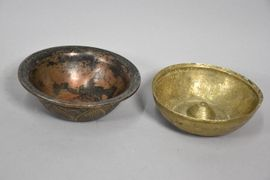
\includegraphics[]{GénéralISTR/Image/bolsmagiques.jpeg}

\includegraphics[]{}


\paragraph{Bol talismanique ou bol magique} coupe de forme circulaire à bords évasés, ombiliquée en laiton anciennement étamé incrustation de pâte noire gravé à l'intérieur de mihrabs, inscriptions en écriture naskh\sn{Le naskh, aussi appelé naskhi ou neskhi  est le style d'écriture le plus répandu pour les langues utilisant l'alphabet arabe. C'est ce style que l'on apprend à l'école et que l'on emploie pour la calligraphie et l'écriture usuelle, manuscrite ou imprimée.} et nasta'liq\sn{Le nastaliq    est un des styles de la calligraphie persane, en alphabet persan, dont l'origine est attribuée à Mir Ali Tabrizi, originaire de Tabriz, au xive siècle} d'invocation religieuse et verset coranique, patine d'usage. Iran XIX-XXe.
Haut. : 4 ; Diam. : 13,5 cm